\NumberThisInToc
\chapter*{Introduction}
%\minitoc
%\vspace{0.5cm}


%\subsubsection{De la dualité onde-corpuscule\ldots}
%\EnFaitNon
{

La description de la lumière a suivi au cours de l'histoire un curieux mouvement de balancier entre une vision \emph{corpusculaire} et une vision \emph{ondulatoire}. Dans la plupart des théories jusqu'au $18\ieme$ siècle, on considère que la lumière est constituée de particules%
%\footnote{Isaac Newton lui-même soutient cette théorie en 1730~\cite{New30}}%
. 
\inlinefig{~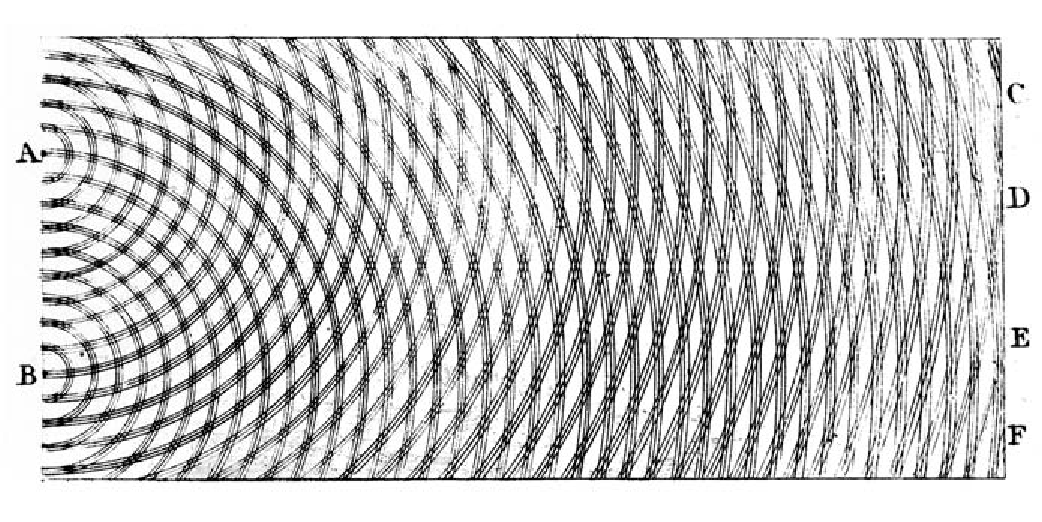
\includegraphics[width=6.75cm]{YoungDiffraction}} 
Un changement de paradigme a lieu à partir de la mise en évidence des phénomènes d'interférences et de diffraction de la lumière par Thomas Young et Augustin Fresnel au début du $19\ieme$ siècle. L'illustration ci-contre de Thomas Young~(1803) représente une expérience d'interférences à double fente. Vers~1850 le modèle ondulatoire devient la norme. La prédiction par Maxwell en~1865 du fait que la lumière est une onde électromagnétique~\cite{Max65}, suivie de la confirmation expérimentale par Hertz en~1888, porte un coup de grâce aux théories corpusculaires de la lumière.

}

\vspace{1ex}
C'est en tentant de modéliser le \termetech{rayonnement du corps noir} qu'en 1900, Max Planck émet l'hypothèse que les échanges d'énergie entre matière et rayonnement sont quantifiés~\cite{Pla01}. Celui-ci pose alors sans le savoir la première pierre de la physique quantique. Presque cinq ans plus tard, Albert Einstein remet en question la nature même du rayonnement électromagnétique en stipulant que la quantification de l'énergie en est une propriété fondamentale~\cite{Ein05}. La notion de \termetech{photon} émerge alors, soulignant une dualité apparemment paradoxale : la lumière semble posséder les propriétés à la fois d'une onde et d'un corpuscule.
C'est le développement de la mécanique quantique, durant les vingt années suivantes, qui va permettre d'interpréter cette double nature.


Louis \dB, durant sa thèse de doctorat~\cite{Bro24} en 1923, formule l'hypothèse selon laquelle 
tout corpuscule matériel possède des propriétés ondulatoires caractérisées par une \lo $\lambdaDB$ qui s'exprime :
\[
\lambdaDB = \frac{h}{p}
\virguleformule
\]
où $h$ est la constante de Planck et $p$ est la quantité de mouvement de la particule. Cette hypothèse généralisait donc aux \emph{particules massive} la dualité onde-corpuscule.

L'expérience de Davisson-Germer, en 1927, apporte la première confirmation expérimentale de l'hypothèse de \dB par l'observation de la diffraction d'électrons par un cristal de nickel~\cite{DaG27}. 
La \lo de \dB étant inversement proportionnelle à la masse et à la vitesse des particules, il est difficile de mettre en évidence le caractère ondulatoire des atomes%
%, à moins de les manipuler à très basse température%
\footnote
{Considérons le cas d'un atome léger, l'hélium, pris dans des conditions de température ambiante. La \lo thermique de \dB est alors:
$
\lambdaDB = \ttfrac{h}{\sqrt{2\,\pi\,m\,\kb\,T}} \approx \SI{0.5}{\angstrom}
,
$
qui est de l'ordre du rayon de l'atome d'hélium. 
}%
.
%
Il faut attendre les années 1980 pour observer la diffraction d'un jet d'atomes issus d'une source à température ambiante~\cite{MGA83,KSS88}.
%diff réseaux~\cite{MGA83}
%diff grating~\cite{KSS88}


\casse


Avec l'apparition des techniques de refroidissement laser~\cite{Phi98,Chu98,Coh98,MeS99} on observe un développement spectaculaire du domaine de l'\termetech{optique atomique}. Cette discipline, dont la référence~\cite{Mey01} présente une introduction détaillée, consiste à tirer parti des propriétés ondulatoires de la matière pour des expériences de diffraction ou d'interférences traditionnellement réalisées avec de la lumière. 

Dans une expérience d'optique atomique, une source d'atomes froids peut être considérée comme l'analogue d'une source lumineuse ayant une faible largeur spectrale.
Toutefois, même à très faible température, les sources atomiques ne sont pas parfaitement cohérentes. 


\section{Quand la matière devient une onde cohérente}

\subsubsection{La lumière laser}

La notion de \termetech{laser} a pris naissance avec le concept d'émission stimulée introduit par Albert Einstein en 1917~\cite{Ein17}. Mais ce n'est qu'en 1953 qu'est conçu le premier \termetech{maser} (l'analogue du laser pour le domaine des micro-ondes)~\cite{GZT55}. %Au cours des six années suivantes, de nombreux scientifiques tels N. G. Bassov, A. M. Prokhorov, Ch. H. Townes (Prix Nobel 1964) et A. L. Schawlow (Prix Nobel 1981) contribuent à développer le formalisme théorique pour décrire le rayonnement maser, puis à adapter leur théorie aux longueurs d'ondes du rayonnement visible. 
%
En 1960, le physicien américain Théodore Maiman obtient pour la première fois une émission laser \emph{pulsée} en utilisant un cristal de rubis comme milieu amplificateur~\cite{MAI60}. Six mois plus tard Ali Javan et ses collaborateurs mettent au point un laser au gaz (hélium et néon) dont l'émission est cette fois-ci \emph{continue}~\cite{JBH61}.

Dans une cavité laser, un nombre macroscopique de photons occupent tous le même mode spatial de propagation et sont cohérents entre eux (même \lo, même phase, même polarisation). 
Chaque photon fait partie d'une seule et même onde macroscopique cohérente. C'est de cette propriété que découle la plupart des applications de la lumière laser : télécommunications, médecine, recherche fondamentale, armement, industrie, etc\ldots

\ifthenelse{\FormatEUE > 0}{}
{\AjouteLigne}

\subsubsection{La \cbe}
En 1924, prolongeant une idée du physicien indien Satyendranath Bose, Albert Einstein formule une autre prédiction théorique : pour un ensemble de particule confinée sans interaction, en dessous d'une certaine température critique, un nombre macroscopique d'atomes s'accumulent dans l'état d'énergie minimale%
\footnote{Cette transition ne peut être effectuée que par une certaine classe de particules, appelées \termetech{bosons}, dont le \termetech{spin} (le moment cinétique intrinsèque) est un multiple entier de $\hbar$.}%
. 
En entrant dans ce régime dit de \termetech{dégénérescence quantique}, les atomes occupent tous, de manière cohérente, une même fonction d'onde macroscopique, formant 
\inlinefigr{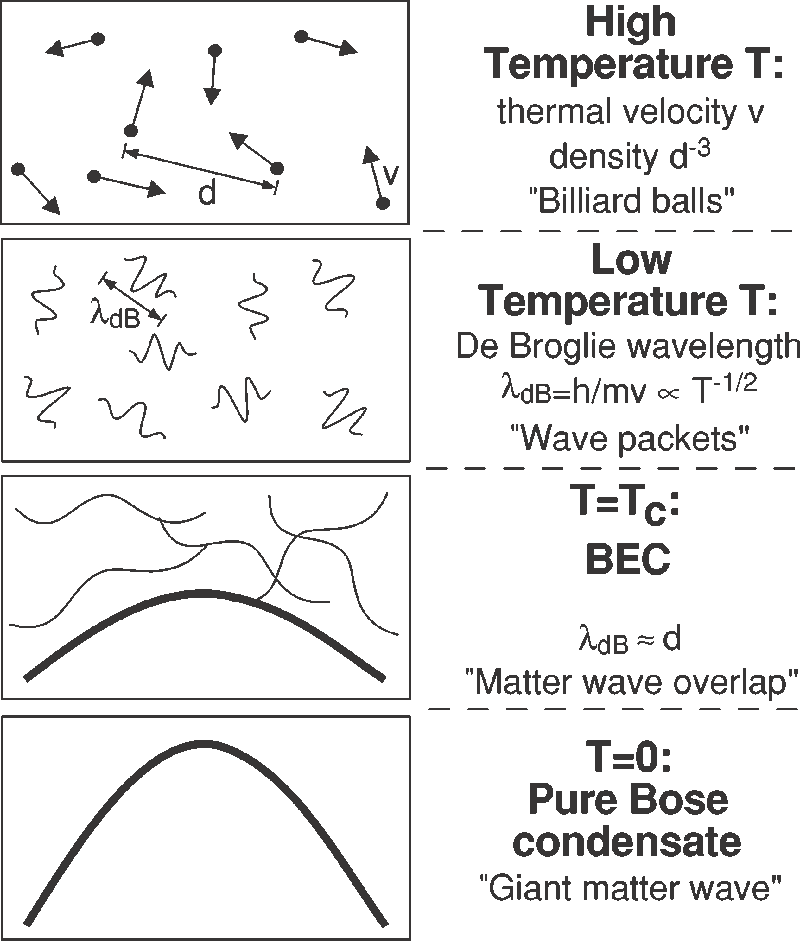
\includegraphics[width=5.5cm]{Ket02}} 
\vspace{-1.5ex}
\noindent
ce qu'on appellera plus tard un \termetech{\bec}. 
Toutefois la \condbe se produit à des températures si basses qu'il est inimaginable en 1924 que l'on puisse l'atteindre un jour.

Plus de 70 ans plus tard, en combinant les techniques de refroidissement laser avec et du \termetech{\rpef}, Eric Cornell, Carl Wieman et Wolfgang Ketterle produisent en 1995 les premiers \becs~\cite{AEM95,DMA95}. Ils obtiennent pour leurs travaux le Prix Nobel en 2001.

L'illustration ci-contre est issue de la \termetech{conférence Nobel} 2001~\cite{Ket02}. Elle schématise la \condbe, qui intervient quand la \lo de \dB devient de l'ordre de la distance entre atomes.
\picskip{0}

\casse

Le caractère cohérent des \bec a été mis en exergue dès 1997 par l'équipe du professeur W.~Ketterle~\cite{ATM97}. 
En 2000, le groupe de T.~Hänsch (Prix Nobel 2005) s'est intéressé à la longueur de cohérence spatiale d'un \bec. Il observe que la longueur de cohérence est, pour une géométrie \tde, de l'ordre de la taille du \becc%
\footnote{Si pour une géométrie \tde la phase de la fonction d'onde est constante sur toute l'extension du \becc, d'autre expériences montrent en revanche que, dans une géométrie \ude, des fluctuations de phase sont observées le long de l'axe longitudinal~\cite{DHR01,RGT03}.}~\cite{BHE00}.

L'analogie entre les photons d'une cavité laser et les atomes d'un \becc est évidente. 
La manipulation d'ondes de matière cohérente ouvre alors de nombreuses perspectives : 
\begin{itemize}
	\item en métrologie, pour mesurer avec une très grande précision des temps, des vitesses de rotation ou des accélérations~\cite{Bor02},
	\item en nano-lithographie, où l'on peut imaginer graver des structures sub-nanométrique par interférences, 
	\item des mesures interférométriques de grandeurs jusqu'alors inaccessible aux systèmes optiques, les atomes étant sensibles à différents champs de force (champ de gravité, champ magnétique,\ldots).
\end{itemize}
Cependant, il faut disposer d'un moyen d'extraire, puis de manipuler les atomes d'un \becc, tout en préservant leur cohérence.

\subsubsection{Le \lat}
%Actuellement, plus d'une trentaine de laboratoires de par le monde disposent d'une expérience de \condbe. 
L'extraction d'ondes de matière cohérente à partir de ces \beccs a d'ores et déjà été réalisée par plusieurs groupes de recherche. Pour ce faire, divers types de coupleur de sortie ont été réalisés:
\def\spppace{\vspace{1ex}}
\def\hpppace{\hspace{-2em}}
\def\sssize{12cm}

\spppace
\inlinefigr{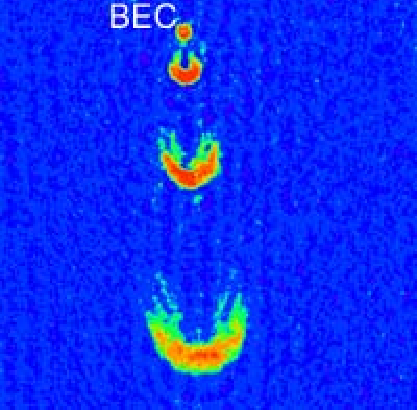
\includegraphics[width=3.5cm]{MAK97a}} 
\hpppace
\begin{minipage}{\sssize}
\begin{ditemize}
	\item en utilisant une impulsion \rf induisant des transitions entre les \snZs, les atomes peuvent passer d'un état piégé magnétiquement à un état non piégé. Un paquet d'ondes de matière cohérente tombe alors sous l'effet de la gravité~\cite{MAK97}. L'illustration ci-contre est issue de la référence~\cite{Ket02}.
\end{ditemize}
\end{minipage}

\spppace
\hpppace
\begin{minipage}{\sssize}
\begin{ditemize}
	\item par un schéma de couplage utilisant des impulsions laser pour effectuer des transition \termetech{Raman}~\cite{HDK99}. Le paquet d'onde de matière est découplé en se voyant communiquer une quantité de mouvement bien contrôlée.
\end{ditemize}
\end{minipage}

\spppace
\inlinefigr{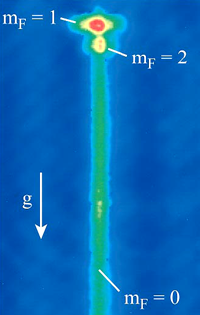
\includegraphics[width=3.5cm]{BHE99a}} 
\hpppace
\begin{minipage}{\sssize}
\begin{ditemize}
	\item il est aussi possible d'obtenir un couplage de sortie continu par application d'une onde \rf. L'extraction \termetech{quasi-continue} peut alors atteindre une durée  de \ms{100}~\cite{BHE99} (voir l'illustration ci-contre). Celle-ci n'est limitée que par le nombre d'atomes initialement présents dans le \becc. Au fur et à mesure que celui-ci se vide, la \rf doit être précisément ajustée afin de maintenir un taux de sortie le plus constant possible.
\end{ditemize}
\end{minipage}

\spppace
\hpppace
\begin{minipage}{\sssize}
\begin{ditemize}
	\item le groupe australien du professeur J.~D.~Close a récemment mis au point une nouvelle méthode d'extraction quasi-continue d'atomes à partir d'un \becc piégé magnétiquement grâce à une paire de faisceaux Raman ~\cite{RFH06}. 
	%La méthode débouche sur un jet de grande brillance pour une durée courte inférieure à 10 ms. Elle requiert toutefois un contrôle très précis des champs magnétiques.
	Ce même groupe affirme qu'il n'est d'ailleurs  pas possible d'augmenter arbitrairement le \fat extrait d'un \becc par une méthode \rf sans impliquer une forte  augmentation des fluctuations d'intensité du \lat~\cite{RMH05}.
	%En effet, augmenter le taux de couplage de sortie du \becc s'accompagne d'une très forte augmentation des fluctuations d'intensité du \lat.
\end{ditemize}
\end{minipage}

\picskip{1}~
\casse

%\spppace
%\hpppace
%\begin{minipage}{\sssize}
%\begin{ditemize}
%	\item 
\noindent
	Dans un piège purement optique l'extraction de l'onde de matière peut s'obtenir en réduisant progressivement la puissance des faisceaux lasers en fonction du temps~\cite{CRG03a}. %Les flux qui en résultent sont très faibles du fait que le \becc contient initialement seulement \val{E4} atomes. Cette technique a l'avantage de ne pas être sensible aux variations des champs magnétiques. 
%\end{ditemize}
%\end{minipage}



De tels dispositifs sont communément désignés par le terme de \emph{\lat}.
%
%\inlinefigl{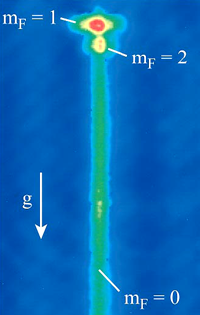
\includegraphics[width=4cm]{BHE99a}} 
%Toujours à l'aide d'une onde \rf, il est possible de mener à bien l'extraction \termetech{quasi-continue} sur une durée pouvant atteindre \ms{100}~\cite{BHE99}.
% 
%Le faisceau d'onde de matière obtenu par cette méthode d'extraction continue possède un flux de quelques millions d'atomes par seconde sur une durée de l'ordre de \ms{100}.
%L'expérience présente un très bon accord avec la théorie développée dans l'article, ainsi qu'avec une étude théorique approfondie réalisée deux ans après dans le groupe d'Alain Aspect~\cite{GBA01}. 
%
%
En toute rigueur, tous les \lats existant à ce jour doivent être qualifiés de \emph{pulsé} car l'extraction de l'onde de matière mène à la déplétion du \becc. Il faut alors en produire un nouveau pour répéter l'opération.
%Un autre défaut majeur de ce type de réalisation de \lat réside dans les \fats moyens très faibles qu'elles produisent, de l'ordre de \val{E4} atomes par seconde. 

S'il a fallu à peine six mois, en 1960, pour passer du laser à rubis pulsé au laser He-Ne continu, on constate que l'obtention d'une onde de matière cohérente, continue et intense reste toujours un défi expérimental, treize ans après l'obtention du premier \becc.

\subsubsection{Propriétés d'un \lat}
Plusieurs expériences ont été réalisées afin d'étudier les caractéristiques des faisceaux d'ondes de matière obtenus par extraction cohérente depuis un \bec. On peut citer des travaux concernant l'étude des propriétés suivantes :
\begin{itemize}
	\item la qualité du faisceau d'un \lat~\cite{LTR01,RGC06},
	\item sa cohérence temporelle~\cite{KHE01},
%La cohérence temporelle mesurée est à la limite de Fourier, plus la durée d'émission est longue, plus la largeur spectrale est faible (ici 700Hz pour une durée d'émission de \ms{1.5}), ce qui traduit une cohérence temporelle parfaite. 
	\item ses propriétés statistiques (fonction de corrélation)~\cite{ORK05}.
\end{itemize}
De plus, il a été démontré qu'un tel faisceau de matière cohérente peut être manipulé à la manière d'une onde lumineuse. \termetech{Réflexion}, \termetech{focalisation}, \termetech{stockage dans un résonateur}; ces termes, habituellement associés à des faisceaux optiques, entrent dans le vocabulaire propres aux \lats~\cite{BKG01}.


\ifthenelse{\FormatEUE > 0}{}
{\AjouteLigne}

\section{Vers le \lat continu à grand \fat}
Le caractère pulsé des \lats que nous avons décrits présente un inconvénient évident pour un certain nombre d'applications. De plus ils ne mettent à disposition qu'un très faible flux moyen d'atomes condensés. C'est en effet cette propriété dont il faut tenir compte pour des applications de type nano-lithographie ou certaines mesures de précision. 

%\ApplicationNumerique%
\Remarque
{
Un \bec ($\approx \val{E5}$ atomes) vidé toutes les 5 secondes (temps typique pour reformer un nouveau \becc) donne un flux moyen de quelques \val{2E4} atomes par seconde. Ce qui signifie, pour donner un ordre d'idée, que le temps nécessaire pour couvrir un millimètre carré d'une monocouche atomique serait d'environ 10 ans \ldots
}
Certaines applications potentielles des \lats nécessiteraient l'obtention de \fats beaucoup plus élevés et, si possible, d'un fonctionnement en continu. 
Pour cela, deux approches semblent possibles :
\begin{itemize}
	\item la première consiste à ré-alimenter le \becc au fur et à mesure de l'extraction de l'onde de matière. Un premier pas dans cette direction a été fait par l'équipe de W.~Ketterle en 2002 au \nomofficiel{MIT}~\cite{CSL02}: un \bec piégé optiquement est périodiquement ré-alimenté par de nouveaux \beccs produits dans une chambre auxiliaire et transportés à l'aide d'une \termetech{pince optique}.
	\item la seconde possibilité consiste à produire un \jatg, puis à y adapter la technique d'\evap afin d'atteindre le \rdq. C'est cette méthode originale, proposée en 2000 par le groupe \nomofficiel{Atome-Froids} du laboratoire Kastler Brossel (ENS)~\cite{MMD00}, qui fait l'objet de ce mémoire de thèse.
\end{itemize}
%D'après une étude théorique effectuée dans ce même groupe, la cohérence spatiale de ce type de laser serait assez faible selon l'axe de propagation ~\cite{CDM00}
%
%\subsubsection{Une nouvelle approche vers un \lat continu et intense}
%Pour cela nous utilisons une approche originale proposée en 2000~\cite{MMD00} et qui consiste à refroidir directement un jet atomique guidé magnétiquement. 
%Le dispositif expérimental dont nous disposons repose sur l'injection périodique, 5 fois par seconde, de nuages d'atomes froids dans un guide magnétique de 4,5 mètres de long. Celui-ci se compose de quatre tubes de cuivre parallèles, refroidis par eau, produisant un champ magnétique quadrupolaires qui guide les atomes de rubidium préparés dans l'état $\EtatFmF{1}{-1}$. Le flux continu est obtenu par le recouvrement spatial des différents paquets atomiques dès les 50 premiers centimètres de propagation dans le guide [13]. Les caractéristiques du faisceau atomique que nous produisons sont les suivantes :
% 	Un flux de \atps{7E9} at / s
% 	Une vitesse moyenne de \cmps{60}
% 	Une température de \microK{600}
% 	Une densité dans l'espace des phases d'environ \val{2E-8}
% 	Un taux de collision moyen par atome de \smun{5}
%
%\subsubsection{Etudes théoriques}
%\cite{CDM00}
%Cet article constitue la première étude théorique qui vise à comprendre les propriétés de cohérence d'un jet continu guidé magnétiquement dans le \rdq. Ces propriétés de cohérence sont étudiées par le biais des fonctions de corrélations longitudinales. Le résultat essentiel porte sur le rôle clé joué par les interactions. En effet, en l'absence d'interactions la fonction de corrélation du deuxième ordre présente un caractère poissonien qui traduit des fluctuations importantes du flux de matière condensée. Ce flux est en revanche stabilisé par la présence d'interactions répulsives entre les atomes. La fonction de corrélation du premier ordre a une décroissance exponentielle avec pour longueur caractéristique quelques longueurs d'onde de \dB thermique pour la température du jet. Cette longueur est relativement faible, de l'ordre de quelques micromètres pour des paramètres expérimentaux typiques. Elle ne fait que refléter les fluctuations de phase présente dans les géométries à dimensions réduites~\cite{DHR01,RGT03}.
%
%\subsubsection{Mise en \oe uvre expérimentale}
%La première étape a consisté en l'alimentation en continu d'un guide magnétique de dimension métrique~\cite{CRA02}, par opposition à l'état de l'art en 2000 où seuls des paquets d'atomes avaient été couplés à des guides de dimension centimétrique. Récemment, le groupe de G. Raithel dans le Michigan~\cite{OMR06} a réalisé une expérience de même nature que celle de l'école normale supérieure. L'objectif est naturellement ensuite de mettre en oeuvre le refroidissement par évaporation. Le premier prérequis est d'atteindre le régime collisionnel. Cette étape a été franchie en 2004 :
%
%\cite{LVG04}
%
%Dans cet article, un jet continu guidé magnétiquement est mis hors équilibre grâce à une onde radio-fréquence. Son retour à l'équilibre thermodynamique sous l'effet des collisions élastiques est étudié par une méthode de spectroscopie radio-fréquence originale.
%
%\cite{LWR05}
%
%Le refroidissement par évaporation à proprement parler est présenté dans cette dernière publication. Les auteurs ont cumulé le long du guide magnétique une dizaine de zones d'évaporation consécutives.
%En ajustant les hauteurs successives de troncature énergétique de la distribution transverse des atomes du jet, ils ont démontré un gain d'un ordre de grandeur sur la densité dans l'espace des phases du jet atomique. Il reste toutefois à gagner 7 ordres de grandeur sur cette dernière quantité pour atteindre le \rdq. La limite imposée au gain en densité dans l'espace des phases résulte du faible nombre de collisions élastiques (~ 20) que chaque atome subit lors de sa propagation dans le guide magnétique. Avec un taux de collisions dix fois plus élevé le \rdq est a priori accessible. Ce groupe étudie actuellement différentes stratégies pour atteindre ce dernier objectif.
%







\casse


\section{Présentation des travaux}% : une nouvelle approche vers un \lat continu et intense}

Le travail réalisé au cours de ma thèse peut se décomposer en trois parties, chacune contenant deux chapitres.
Les différents thèmes de recherche qui seront présentés dans ce mémoire de thèse ont tous donné lieu à la rédaction d'un article scientifique~\cite{LWR05,LRW06,RWC06,RLC06,CKR08,RLW07,CJK08,ReG08}. Les références et résumés de ces articles sont réunis dans l'annexe~\nref{annexe:Articles} (\vpageref{annexe:Articles}).

\ifthenelse{\FormatEUE > 0}{}
{\AjouteLigne}

\subsubsection{Première partie: \TitrePartieUn}
%Cette partie traitera de la formation et de l'évaporation d'un \jatgm:
\begin{ditemize}
%
	\item le chapitre \ref{chap:JetAtomique} introduit les concepts qui vont servir de supports aux différentes analyses liées au guidage magnétique. Nous y présenterons notamment le \setup tel qu'il existait à mon arrivée dans l'équipe de \dgo. L'étude du \jatgm avait alors déjà montré que le \tcolel était suffisant pour pouvoir mettre en \oe uvre le \rpef. \`A l'issue de ma première année de thèse, nous avons ainsi pu mettre en évidence un gain d'un ordre de grandeur sur la densité dans l'espace des phases du jet~\cite{LWR05}.
%
	\item le chapitre \ref{chap:Ceramique} présente une technique efficace permettant de mener à bien l'\evap d'un \jatmg. Nous avons adapté le principe d'élimination d'atomes énergétiques au contact d'une surface matérielle~\cite{HMO03} à notre \setup. 
%
\end{ditemize}
Dans la première partie nous soulignerons le fait que l'évaporation d'un \jat est une tâche fondamentalement plus ardue que celle mise en \oe uvre habituellement sur un nuage piégé. Afin de pouvoir atteindre le \rdq, nous conclurons sur la nécessité de développer de nouveaux outils permettant d'augmenter le nombre de \colels au sein du jet. 


\subsubsection{Deuxième partie: \TitrePartieDeux}
%Cette partie traitera de la manipulation et du refroidissement de \pats dilués, lors de leur propagation dans le \gm:
%Le paramètre physique qui nous limite est le nombre moyen $\Ncol$ de collisions subies par un atome au cours de sa propagation. Une estimation montre que si nous pouvions disposer d'un nombre dix fois plus élevé de collisions (soit $\Ncol\approx200$), le \rdq serait alors accessible.
\begin{ditemize}
%
	\item le chapitre \ref{chap:MiroirMobile} décrit la mise en \oe uvre d'une technique de ralentissement de \pats guidés par réflexion sur un \mimamo. Nous y démontrons l'efficacité de cette méthode ainsi que l'intérêt qu'elle présente dans le contexte de la production d'un \jatuf continu et dense~\cite{RLC06}. Nous serons d'ailleurs amenés à comparer l'action du \mimo sur les \ps avec celle d'un \termetech{démon de Maxwell}~\cite{ReG08}.
%
	\item le chapitre \ref{chap:Convoyeur} présente une technique originale permettant de capturer les \pats guidés dans un \tpm \tds fait d'aimants permanents~\cite{LRW06}. Nous expliciterons, avec l'appui de simulations numériques, les mécanismes physiques à l'\oe uvre dans ce problème de transport. 
Nous y présenterons enfin les résultats démontrant le transport ainsi que le refroidissement des paquets piégés dans le \tpm.

%
\end{ditemize}
 
%\pagebreak
 
\subsubsection{Troisième partie: \TitrePartieTrois}
%Dans cette dernière partie, nous étudierons la possibilité de produire, manipuler et étudier des \nats denses:
\begin{ditemize}
%
	\item le chapitre \ref{chap:PiegeDipolaire} présente une méthode de production de \pats très denses grâce à un piège optique à force dipolaire. Nous y traiterons aussi de la mise en mouvement de ces \ns. Un modèle analytique simple nous servira de support pour présenter les résultats expérimentaux liés à l'optimisation du transport~\cite{CKR08}.
%
	\item le chapitre \ref{chap:Imagerie} décrit un nouveau protocole d'imagerie que nous avons développé lors de ma deuxième année de thèse. En effet, les deux techniques prédominantes pour faire l'image d'ensembles atomiques dilués, à savoir l'\termetech{imagerie par absorption à faible intensité} et l'\termetech{imagerie par fluorescence}, s'avèrent peu fiables lorsqu'il s'agit de traiter des \ns dont la \pro excède \val{4}-\val{5}.
Notre protocole permet de résoudre les structures de \nats denses et donne accès à des mesures quantitatives et précises~\cite{RLW07}. 
%
\end{ditemize}
 


%\subsubsection{Condensation de Bose~\cite{CJK08}}
%Précisons enfin qu'en utilisant une configuration de faisceaux croisés  avec notre laser de puissance, nous avons récemment réalisé un \bec. Celui-ci contient typiquement \val{E5} atomes et est réaliser en 6 secondes. Nous pouvons contrôler précisément l'état interne des atomes qui le compose en utilisant une méthode de distillation de spin par application de gradients de champs magnétiques au cours de l'évaporation. Cette technique de contrôle des états internes a été mise à profit pour extraire du \becc un \lat guidé optiquement~\cite{CJK08}.


